\documentclass{article}
\usepackage{tikz}
\usetikzlibrary{positioning}
\begin{document}
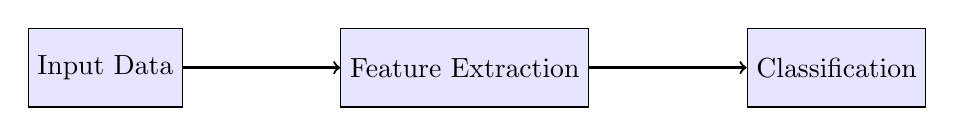
\begin{tikzpicture}[node distance=2cm, auto, every node/.style={draw, rectangle, fill=blue!10, minimum height=1cm, text centered}]
\node (A) {Input Data};
\node (B) [right=of A] {Feature Extraction};
\node (C) [right=of B] {Classification};
\draw[->, thick] (A) -- (B);
\draw[->, thick] (B) -- (C);
\end{tikzpicture}
\end{document}